\chapter{Implementation}
\label{ch:implementation}

\section{Software}
\subsection{mbed LPC1768}
\label{subs:mbed}
The mbed LPC1768 task is to consecutively wake up and initialise the VL53L0X sensors, read the ranging data, and send it forward to the pixhawk. To operate the sensor the use of the sensor's API is required in which several C functions are predefined. To wake up the VL53L0X sensor the XSDN line (\cref{fig:schematics}) is set from low to high and a I2C bus address is allocated. After a successful boot of the sensors, initialization starts and the calibration data is loaded. The calibration of the sensors is performed during the final module test at STMicroelectronics, thus the customer has to simply load the calibration data. In case cover glass is used on top of the VL53L0X, the sensor has to be recalibrated as explained in the user manual. Ensuing a successful initialisation, the ranging measurement is started. We programmed mbed LPC1768 to only conduct a measurement if addressed by the pixhawk (\cref{alg:px4}). 

\begin{algorithm}
	\caption{VL53L0X measurement}\label{alg:px4}
	\begin{algorithmic}[1]
		\Procedure{RANGING}{ }
		\State Set all XSDN lines to low
		\For{every VL53L0X sensor}
		\State Set XSDN line to high
		\State Allocate sensor to I2C bus address
		\EndFor
		\For{every VL53L0X sensor}
		\State Initialise 
		\State Load calibration data
		\EndFor
		\State Start Measurement
		\For{all time}
		\If{LPC1768 is addressed from pixhawk}
		\State Conduct measurement
		\EndIf
		\EndFor
		\EndProcedure
	\end{algorithmic}
\end{algorithm}

\subsection{Pixhawk}
\label{subs:pixhawk}
In the pixhawk firmware we've added the driver \textit{VL53L0X}, the topics \textit{VL53L0X} and \textit{pf}, and the module \textit{potential\_field}. The only task of the driver \textit{VL53L0X} is to continuously read the ranging data sent by the microcontroller and publish the data to the topic \textit{VL53L0X}. The topic is subscribed by the module \textit{potential\_field} in which attitude corrective angles $q_{pf}$ are calculated w.t.h. of a potential field (\cref{eq:angle sp}). We have included a upper threshold to the corrective angles. These corrective angles are published to the topic \textit{pf}. The multi-copter attitude controller (module \textit{mc\_att\_control}) subscribes to the topic \textit{pf}. In the attitude controller, the corrective attitude angles $\Omega_{corr}$ are added to the attitude set-points $\Omega_{sp}$ (\cref{eq:new sp} \cref{alg:px4}). Driver \textit{VL53L0X} and Module \textit{potential\_field} start automatically when the pixhawk is booted. If the LPC1768 is running during the boot of the pixhawk, the LPC1768 has to be reset by pushing the button on top of the microcontroller. Otherwise, the pixhawk is not able to read the ranging measurement correctly. 

\begin{algorithm}
	\caption{Pixhawk}\label{alg:px4}
	\begin{algorithmic}[1]
		\Procedure{PIXHAWK}{ }
		\State Driver  \textit{VL53L0X} reads ranging data from I2C bus 
		\State Driver  \textit{VL53L0X} publishes ranging data to topic \textit{VL53L0X}
		\State Module \textit{potential\_field} subscribes to topic \textit{VL53L0X}
		\State $y_{data}\gets \text{ranging data from topic \textit{VL53L0X}}$
		\State $\Omega_{corr} \gets \text{corrective attitude angles computed with a potential field}$ (\cref{eq:angle sp})
		\State Module \textit{potential\_field} publish $\Omega_{corr}$ to topic \textit{pf}
		\State Module \textit{mc\_att\_controller} subscribes to topic \textit{pf}
		\State $\Omega_{sp}'\gets \Omega_{corr}+\Omega_{sp}$ \Comment{new set-point calculated}
		\EndProcedure
	\end{algorithmic}
\end{algorithm}

\section{Hardware}
The avoidance system is powered through the battery of the MAV, which, in our case, outputs around \unit[12]{V} to our system. We protect our system from overcurrent with a fuse and from switching polarities with a diode. A buck converter is used to step down the voltage to \unit[5]{V}, the input voltage of the mbed LPC1768. With a second buck converter we further step down the voltage to \unit[3.3]{V}, the supply voltatge of VL53L0X ranging sensors and from where the I2C bus is pulled up. All VL53L0X sensors are connected to the same I2C bus. The mbed LPC1768 is the master device on the bus. The pixhawk and the mbed LPC1768 are on a separate I2C bus on which the pixhawk is the master device. The XSDN line is used for shutting down and waking up the VL53L0X devices. If the line is set to low the VL53L0X is shut down and if the line is set to high the VL53L0X is waken up. This is used to set the I2C bus addresses of the VL53L0X sensors (\cref{fig:schematics}). We solder the parts on PCB (\cref{fig:pcb}) and 3D printed a case for the system. The case is mounted on the MAV (\cref{fig:system}). 
\begin{figure}
	\centering
	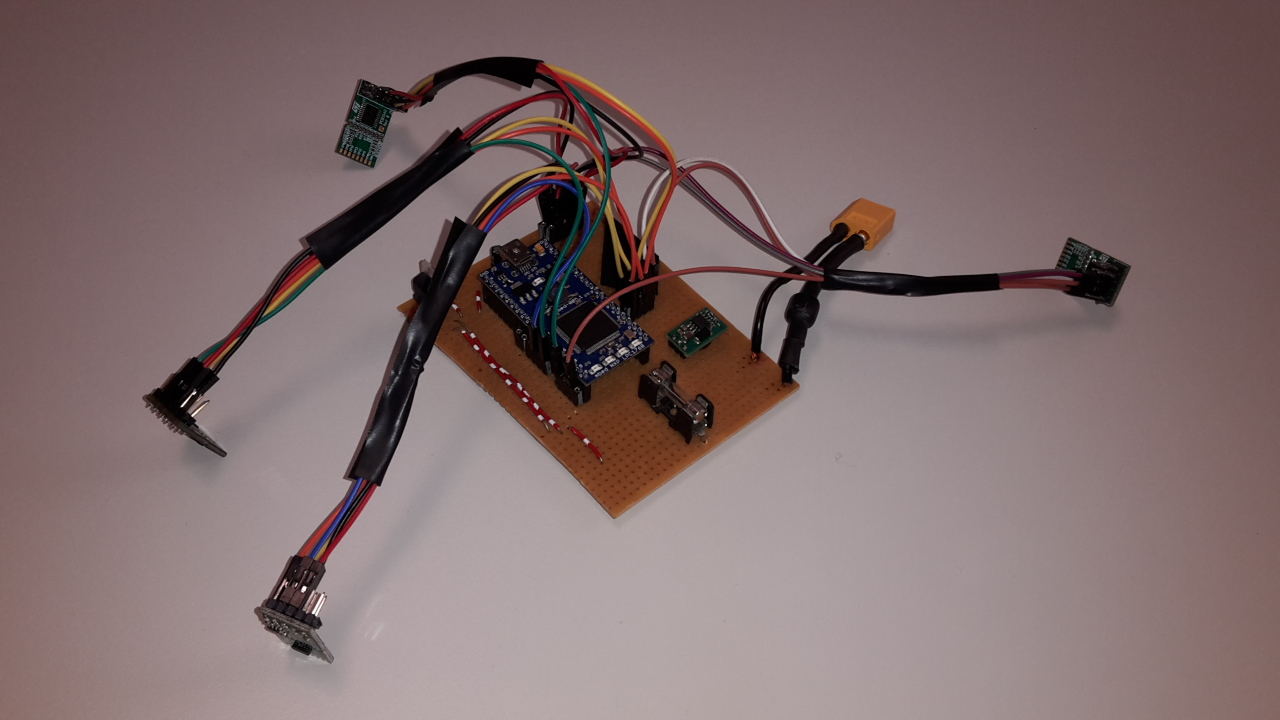
\includegraphics[width=\linewidth]{pictures/pcb.jpg}
	\caption{System soldered on a PCB board.}
	\label{fig:pcb}
\end{figure} 
\begin{figure}
	\centering
	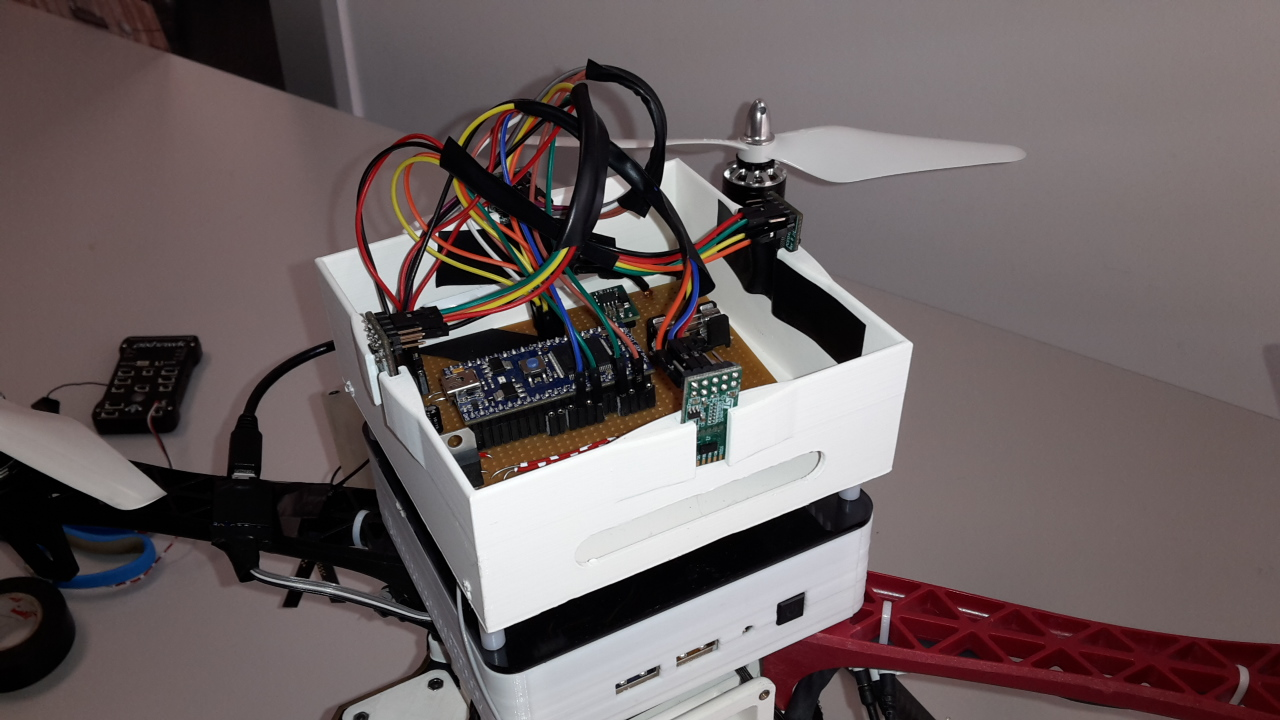
\includegraphics[width=\linewidth]{pictures/system.jpg}
	\caption{System mounted on the platform.}
	\label{fig:system}
\end{figure}
\begin{landscape}
	\begin{figure}
		\centering
		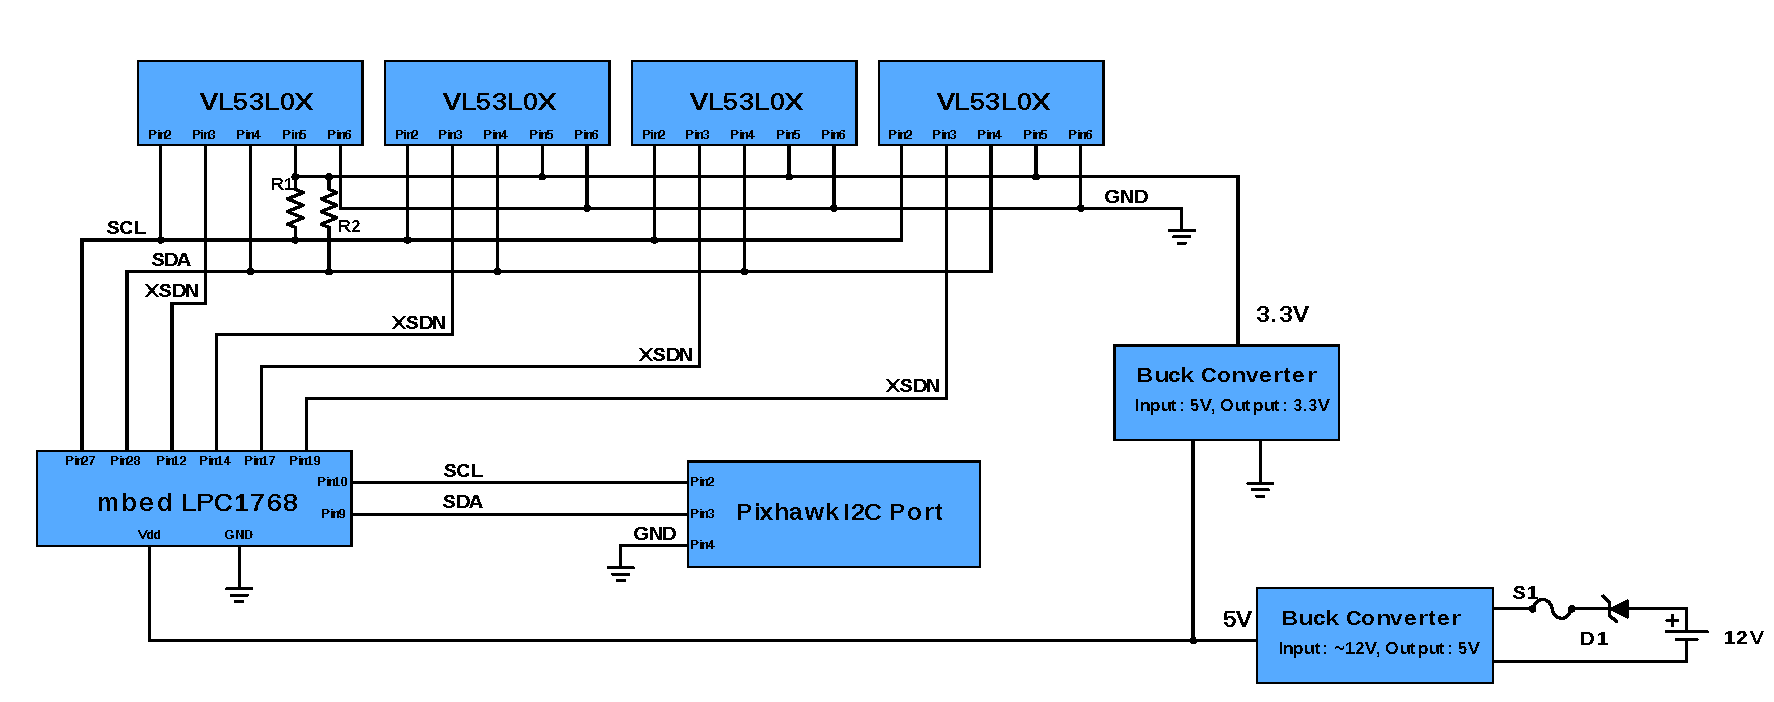
\includegraphics[width=\linewidth]{pictures/wire_schematic.pdf}
		\caption{Schematic of the avoidance system. Resistors $R1=R2=\unit[10]{k\Omega}$, Fuse breaking capacity $S1=\unit[1]{A}$}
		\label{fig:schematics}
	\end{figure}
\end{landscape}




